\subsection{Triển khai Hệ thống Gợi ý}
\label{subsec:recsys_implementation_paragraph} % Label mới

Hệ thống VieVu triển khai hai cơ chế gợi ý chính để đề xuất địa điểm cho người dùng. Mục này trình bày chi tiết việc triển khai kỹ thuật cho cả hai cơ chế: gợi ý địa điểm liên quan dựa trên nội dung (Content-Based) và gợi ý địa điểm chính dựa trên Neural Network (Hybrid).

\subsubsection{Gợi ý Địa điểm Liên quan (Content-Based)}
\label{subsubsec:cb_recsys_impl_paragraph_final} % Label mới

Hệ thống gợi ý địa điểm liên quan hoạt động bằng cách kết hợp điểm đánh giá chất lượng/phổ biến nội tại của địa điểm với độ tương đồng về mặt nội dung văn bản. Đầu tiên, một điểm số nội tại ($Score_{Item}$) cho mỗi điểm tham quan được tính toán. Điểm này dựa trên điểm đánh giá trung bình có trọng số ($Score_{WeightedAvg}$) được làm mượt bằng công thức:
$$Score_{WeightedAvg} = \frac{R \times v + C \times m}{v + m}$$
Trong đó $R$ là điểm trung bình gốc, $v$ là số lượt đánh giá, $C$ là điểm trung bình toàn cục, và $m$ là ngưỡng tối thiểu. Sau đó, giá trị $Score_{WeightedAvg}$ và \texttt{hot\_score} được chuẩn hóa về thang [0, 1] ($ScaledWeightedAvg$, $ScaledHotScore$) và kết hợp thành $Score_{Item}$ cuối cùng với trọng số $w_{hs}=0.6, w_{wa}=0.4$:
$$Score_{Item} = w_{hs} \times ScaledHotScore + w_{wa} \times ScaledWeightedAvg$$
% (Tham khảo mã nguồn tại Đoạn mã \ref{lst:score_calculation}) % <<< Placeholder

Tiếp theo, nội dung văn bản của các địa điểm được tiền xử lý, tổng hợp thành trường \texttt{bag\_of\_words} và vector hóa bằng \texttt{TfidfVectorizer} từ Scikit-learn~\cite{sklearn_lib} (có loại bỏ từ dừng tiếng Việt) để tạo ma trận TF-IDF. Độ tương đồng nội dung giữa hai địa điểm (vector $\vec{a}$ và $\vec{b}$) được đo bằng Cosine Similarity và kết quả là ma trận độ tương đồng \texttt{cos\_sim} giữa các cặp địa điểm. % (Tham khảo tại Đoạn mã \ref{lst:tfidf_cosine_code}) % <<< Placeholder
% $$\text{Cosine Similarity}(\vec{a}, \vec{b}) = \frac{\vec{a} \cdot \vec{b}}{\|\vec{a}\| \|\vec{b}\|}$$

Cuối cùng, hàm gợi ý \texttt{get\_related\_attractions} được triển khai. Hàm này nhận ID địa điểm đang xem, lấy $Score_{Item}$ và độ tương đồng nội dung ($Similarity$) từ \texttt{cos\_sim}, rồi tính điểm gợi ý cuối cùng ($Score_{Final}$) bằng cách kết hợp chúng với trọng số $w_{sim}$ (ví dụ: 0.7):
$$Score_{Final} = w_{sim} \times Similarity + (1 - w_{sim}) \times Score_{Item}$$
Top N địa điểm có $Score_{Final}$ cao nhất (trừ địa điểm gốc) được trả về thông qua API endpoint của FastAPI. % (Tham khảo tại Đoạn mã \ref{lst:related_attractions_func}) % <<< Placeholder

\subsubsection{Gợi ý Địa điểm Chính (Neural Network - Hybrid)}
\label{subsubsec:nn_recsys_impl_paragraph_final} % Label mới

Hệ thống gợi ý chính của VieVu, nhằm đề xuất địa điểm cá nhân hóa, được xây dựng dựa trên mô hình Neural Network (NN) theo cách tiếp cận Hybrid, sử dụng thư viện TensorFlow và Keras~\cite{tensorflow_lib, keras_lib}. Mô hình này dự đoán mức độ phù hợp (rating dự đoán) dựa trên sự kết hợp của ba nguồn thông tin: đặc trưng người dùng (User Features từ khảo sát/hành vi), đặc trưng địa điểm (Item Features gồm thuộc tính số và OHE loại hình), và dữ liệu đánh giá giả lập.

Quá trình chuẩn bị dữ liệu bao gồm tải dữ liệu đặc trưng cho khoảng 3500 người dùng và 1006 địa điểm. Do hạn chế dữ liệu rating thực tế, bộ dữ liệu huấn luyện (\texttt{user\_ratings\_data.csv}) được tạo giả lập bằng cách phân phối ngẫu nhiên điểm rating cho cặp (user, item) dựa trên thống kê gốc (\texttt{avg\_rating}, \texttt{rating\_count}) của địa điểm. Dữ liệu đặc trưng và rating giả lập sau đó được kết hợp và chia thành tập huấn luyện (90%) và kiểm thử (10%).

Mô hình NN được thiết kế theo kiến trúc two-tower song song. Nhánh người dùng và nhánh địa điểm nhận đầu vào là các vector đặc trưng tương ứng, mỗi nhánh đi qua hai lớp Dense (128 và 64 nơ-ron, ReLU). Output từ hai nhánh được ghép nối (Concatenate), đi qua một lớp Dense (64 nơ-ron, ReLU) và lớp Dense output cuối cùng (1 nơ-ron, 'linear') để dự đoán rating. Chi tiết thiết lập các lớp mạng được thể hiện trong Đoạn mã~\ref{lst:nn_model}. % (Sơ đồ kiến trúc có thể xem tại Hình~\ref{fig:nn_arch}) % <<< Placeholder

\lstset{language=python}
\begin{lstlisting}[
    caption=Thiết lập các lớp chính của mô hình Neural Network,
    label=lst:nn_model,
    captionpos=t,
    belowcaptionskip=10pt,
    basicstyle=\small\ttfamily,
    breaklines=true,
    showstringspaces=false,
    inputencoding=utf8]
    # User branch
    user_layer = Dense(128, activation="relu")(input_user)
    user_layer = Dense(64, activation="relu")(user_layer)
    # Attraction branch
    attraction_layer = Dense(128, activation="relu")(input_attraction)
    attraction_layer = Dense(64, activation="relu")(attraction_layer)
    # Merge and predict
    merged = Concatenate()([user_layer, attraction_layer])
    merged = Dense(64, activation="relu")(merged)
    output = Dense(1, activation="linear")(merged)
    
\end{lstlisting}

Mô hình được huấn luyện để tối thiểu hóa Mean Squared Error (MSE) giữa rating dự đoán và rating giả lập, sử dụng optimizer Adam (learning rate 0.001) và theo dõi Mean Absolute Error (MAE). Quá trình huấn luyện diễn ra trong 30 epochs với batch size 32. Kết quả huấn luyện được trực quan hóa trong Hình~\ref{fig:mae} cho thấy mô hình học được từ dữ liệu (Loss và MAE đều giảm) và đạt MAE khoảng 0.64 trên tập kiểm chứng, mặc dù có dấu hiệu overfitting. Mô hình với trọng số tốt nhất được lưu lại. % <<< NHỚ THAY LABEL FIG ĐÚNG !!!
    \begin{figure}[H]
        \centering
        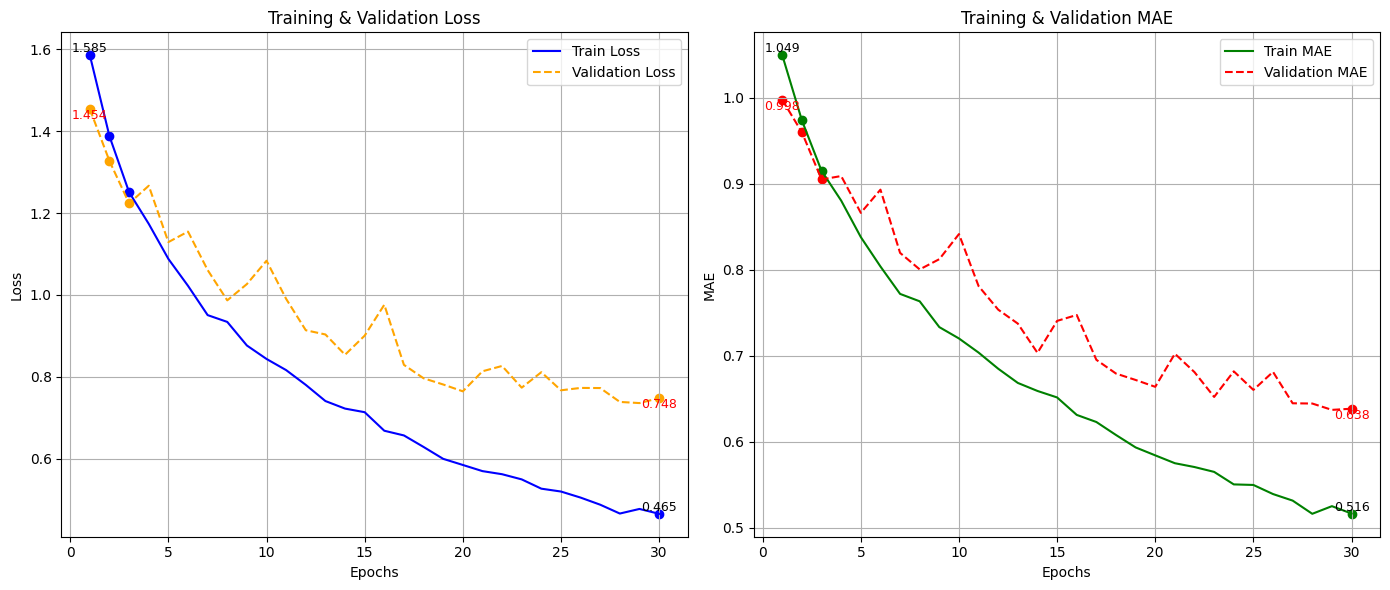
\includegraphics[width=\textwidth]{figures/c4/128.png} % Đường dẫn tới file ảnh của bạn
        \caption{Hiệu suất mô hình qua độ đo MAE và Loss trong quá trình huấn luyện.} % Cập nhật caption
        \label{fig:mae} % Giữ nguyên label nếu bạn đã dùng
    \end{figure}

Như vậy, việc triển khai hệ thống gợi ý địa điểm chính của VieVu đã hoàn thành thông qua việc xây dựng và huấn luyện mô hình Neural Network Hybrid. Bằng cách kết hợp thông tin đặc trưng và tín hiệu học hỏi từ dữ liệu rating giả lập, mô hình được tối ưu hóa để dự đoán mức độ phù hợp. Hệ thống gợi ý cuối cùng được tích hợp vào API server, sẵn sàng cung cấp các đề xuất địa điểm cá nhân hóa cho người dùng.
